\chapter{Software}

    \section{Funcionamiento del Sistema de Control}
    
        \subsection{Introducción}
        
            El sistema de control del proyecto es el encargado de administrar los periodos de carga y descarga de la batería, optimizando su uso en función de los datos recogidos en tiempo real por los distintos sensores que lo integran, distintos datos en formato analógico de la batería, que son sensados para luego ser digitalizados y enviados a la aplicación móvil del usuario.\par
            Esta etapa forma el núcleo lógico del sistema, protagonizada por una RP2040-Zero, ejerce como nexo entre los componentes analógicos y nuestra aplicación.\par
            El microcontrolador se encuentra programado en C, un lenguaje que gracias a su bajo nivel, podrá ser ejecutado por el microcontrolador a una velocidad adecuada.\par
            
        \subsection{Datos obtenidos}
        
            Esta placa cuenta con 2 tipos de sensor principales, que trabajando en conjunto entregan los datos del funcionamiento en tiempo real de la batería y del sistema, información suficiente para continuar con su control.\par
            
            \subsubsection{Encoder Rotativo Incremental}
            
                Encargado de brindarle información al sistema sobre la posición y la velocidad angular, datos que utilizará el sistema para calcular la cantidad de vueltas y la dirección en la que rota el motor. Posee una gran precisión en sus respuestas por la cantidad de pulsos que envía por revolución. Nos permite calcular el porcentaje de carga de la batería, mientras nos brinda los datos para prevenir el funcionamiento errático del sistema.\par
                Para más información sobre este componente en concreto revisar el Apéndice C, y más específicamente la Figura C.3.\par

                \subsubsubsection{Funcionamiento del Encoder}
                \label{fde}
                
                    El encoder basa su funcionamiento en dos señales digitales A y B, estas son generadas en cada pulso y están desfasadas 90° entre sí. Cuando el encoder está alimentado, comienza a enviar pulsos, mismos que variarán cuando el motor esté en movimiento. Para decodificar esta sucesión de pulsos, utilizamos la lectura en cuadratura. Este método basa su funcionamiento en la detección de cambios o transiciones entre las señales A y B.\par
                    Analizando dicha sucesión, este sistema busca detectar el momento en el que se complete un \textbf{ciclo} o \textbf{vuelta}, una sucesión de 4 estados en los que:\par
                    
                    \begin{itemize} [label=•]
                        \setlength{\itemindent}{1.5em}
                        
                        \item A sube (0 a 1)
                        \item B sube (0 a 1)
                        \item A sube (1 a 0)
                        \item B sube (1 a 0)
                    \end{itemize}
                    
                    Es importante observar que hacemos énfasis en el estado anterior de cada señal, ya que lo que realmente nos interesa es la transición entre un estado y otro.\par
                    Nuestro sistema utiliza un contador \texttt{\textbf{counter}} para llevar registro de las transiciones que efectúan las señales del encoder, este se incrementa a medida que se presentan las variaciones que nos interesan. A continuación, presento una serie de estados en los que observaremos el ciclo mencionado anteriormente y el uso del contador en él\par

                    \begin{table}[H]
                        \centering
                        \begin{tabular}{|c|c|c|c|c|c|c|}
                            \hline
                             N° & Estado Anterior A & Estado Anterior B & Estado Actual A & Estado Actual B & Acción & Contador\\
                             \hline
                             1 & 0 & 0 & 0 & 0 & - & -\\
                             \hline
                             2 & 0 & 0 & 1 & 0 & A sube & +1 (\texttt{\textbf{counter}})\\
                             \hline
                             3 & 1 & 0 & 1 & 0 & - & -\\
                             \hline
                             4 & 1 & 0 & 1 & 1 & B sube & -\\
                             \hline
                             5 & 1 & 1 & 0 & 1 & A baja & -1 (\texttt{\textbf{counter}})\\
                             \hline
                             6 & 0 & 1 & 0 & 0 & B baja & -\\
                             \hline
                        \end{tabular}
                        \caption{Tabla de Verdad para Encoder Rotativo en Cuadratura}
                        \label{tab:s1}
                        \end{table}
                        
                        Observamos que:\par
                        \begin{itemize} [label=•]
                            \setlength{\itemindent}{1.5em}
                            
                            \item Cuando ambos pulsos son iguales, no hay cambios en el \texttt{counter} (Estados 1 y 3).
                            \item El incremento del \texttt{counter} (\texttt{counter ++}) ocurre cuando A aumenta y A se mantiene (Estado 2).
                            \item La reducción del \texttt{counter} (\texttt{counter --}) ocurre cuando B aumenta y A se mantiene (Estado 4)
                            \item  Cuando cualquiera de las variables baja a 0 mientras la otra se mantiene, no hay cambios en el \texttt{counter} (Estados 5 y 6).
                        \end{itemize}
                        
                    El incremento en el counter implica giro en sentido horario, su reducción será giro en sentido antihorario.\par
                    Teniendo en cuenta la cantidad de pulsos que emite nuestro encoder por cada revolución, podremos calcular la cantidad de vueltas realizadas por el motor, y en consecuencia el porcentaje de carga de la batería; més específicamente los datos detallados a continuación.\par

                \subsubsubsection{Datos obtenidos por el Encoder}
                    El encoder de nuestro sistema se encuentra conectado al eje del motor generador que mueve la carga de la batería. El encoder nos brinda información angular sobre la posición del eje del motor y las vueltas que realizó.\par
                    Conociendo la cantidad de vueltas que equivalen a un recorrido completo de la batería, podremos conocer el punto al que se encuentra el peso durante todo su funcionamiento.\par
                    
                    \begin{itemize} [label=•]
                \setlength{\itemindent}{1.5em}
                        \item Si el peso se encuentra muy cerca del límite inferior, \textbf{NO} podrá descargarse la batería.
                        \item Si el peso está muy cerca del límite superior, el mismo \textbf{NO} podrá seguir subiendo con la carga de la batería.\par
                    \end{itemize}
                    
                    Estos factores son cruciales porque impiden un posible fallo mecánico de la batería, uno que podría derivar en fuertes daños al dispositivo, sus alrededores y seres circundantes.\par
                    Aparte de los riesgos potenciales que podemos prevenir, nos encontramos en la necesidad de controlar la carga y descarga de la batería, conocer el porcentaje de carga en el que se encuentra y asegurarnos de brindarle esta información al usuario. Con los datos que nos brinda el encoder podemos calcular el porcentaje de carga de la batería, ya que:\par

                    \begin{equation}
                        Porcentaje_{Carga} = \frac{\texttt{lap\_counter}}{\texttt{COMPLETE\_LAPS}} \times 100
                    \end{equation}
                    
                    Donde:\par
                    \begin{itemize} [label=•]
                \setlength{\itemindent}{1.5em}
                
                        \item \texttt{COMPLETE\_LAPS} es la cantidad de vueltas que necesita la batería para completar el recorrido.
                        \item \texttt{lap\_counter} es la cantidad de vueltas que realizó el motor, se actualiza constantemente, cuando realiza vueltas en sentido horario el contador aumenta, y cuando las realiza en sentido antihorario decrece.
                    \end{itemize}
                    
            \subsubsection{INA219}
                El sistema cuenta con 4 sensores INA219. Cada sensor se encuentra midiendo distintos parámetros, con la finalidad de asegurarle al sistema de control valores actualizados de corriente y tensión; de esta forma, el sistema podrá informar al usuario sobre sus acciones a nivel energético, mientras administra la carga y descarga de la batería de forma óptima en tiempo real.\par
                Para más información sobre este componente en concreto revisar el Apéndice C, y más específicamente la Figura C.2.\par

                \subsubsubsection{Funcionamiento del INA219}
                    Estos sensores tienen un principio de funcionamiento muy simple, cuentan con una resistencia de shunt (una resistencia cuyo valor es muy bajo) conectada en serie a la carga.\par
                    El circuito obtiene la diferencia de potencial eléctrico entre sus terminales V+ y V- (donde se encuentra conectada la carga) y conoce el valor de la fuente de alimentación del circuito, por lo tanto podrá obtener el valor de la V de shunt.\par
                    
                        \begin{equation}
                            V_{Shunt} = V_{Total} - V_{Carga}
                        \end{equation}

                    El valor de la tensión de Shunt será muy bajo (suele ser menor a 50mV). El sensor lo que busca es obtener este valor para, utilizando la Ley de Ohm, obtener el valor de corriente.\par

                    \begin{equation}
                        I_{Shunt} = \frac{V_{Shunt}}{R_{Shunt}}
                    \end{equation}

                    Para hacer este cálculo, el valor de Vshunt tiene que estar en formato digital, por este motivo el módulo INA219 tiene su propio ADC integrado. Dentro de las configuraciones que solicitan los módulos encontramos los rangos de revolución del ADC interno. De acuerdo a la cantidad de bits que solicitemos, tendremos mayor o menor precisión en los resultados de las medidas; mientras más bits tendremos más precisión, pero también tomará más tiempo el proceso.\par

                    \begin{table}[H]
                        \centering
                        \begin{tabular}{|c|c|}
                        \hline
                            Resolución (bits) & Tiempo de Conversión\\
                        \hline
                             9 bits & 84 $\mu s$ \\
                        \hline
                            10 bits & 148 $\mu s$\\
                        \hline
                            11 bits & 276 $\mu s$\\
                        \hline
                            12 bits & 532 $\mu s$\\
                        \hline
                        \end{tabular}
                        \caption{Tabla de resolución del ADC}
                        \label{tab:s2}
                    \end{table}

                    Una señal tan pequeña (menor a 50mV) contará con muy poco porcentaje de resolución efectiva. La solución que nos propone el mismo módulo es amplificar la señal, dentro de los parámetros de configuración nos encontramos con 4 opciones de ganancia para la $V_{Shunt}$:\par

                    \begin{table}[H]
                        \centering
                        \begin{tabular}{|c|c|}
                        \hline
                            Ganancia & Máximo $V_{Shunt}$ medible\\
                        \hline
                             1x & ±320 mV \\
                        \hline
                            2x & ±160 mV\\
                        \hline
                            4x & ±80 mV\\
                        \hline
                            8x & ±40mV\\
                        \hline
                        \end{tabular}
                        \caption{Tabla de Ganancias}
                        \label{tab:s3}
                    \end{table}
                    
                    Cada valor de ganancia tiene un amplificador asociado, cada uno cuenta con sus propias características, su valor de ganancia y un valor máximo absoluto. Es importante asegurarnos de no exceder dicho valor porque causaría una saturación en la salida del amplificador, resultando en una pérdida de datos y una lectura incorrecta.\par
                    Una vez calculado el valor de corriente de shunt, podremos suponer que este es el mismo que circula por el resto de la rama, incluyendo a la carga.\par

                    \begin{equation}
                        I_{Shunt} = I_{Carga}
                    \end{equation}
                    
                    El valor de corriente se encuentra en formato digital y listo para ser enviado.\par
                    El módulo de INA219 cuenta con un puerto de comunicación i2c. Estos sensores permiten el uso en simultáneo de hasta 16 dispositivos INA219 conectados en el mismo puerto i2c. Dicha función es posible porque los datos enviados se encuentran encabezados por un byte de dirección, dato que se puede configurar desde los pines A1 y A0 de los módulos. Al conectar estos pines a distintos puntos, podremos obtener distintas direcciones, a continuación podemos observar las distintas posibilidades que nos ofrece.\par

                    \begin{table}[H]
                        \centering
                        \begin{tabular}{|c|c|c|}
                        \hline
                            \texttt{A1} & \texttt{A0} & \texttt{SLAVE ADDRESS}\\
                        \hline
                             \texttt{GND} & \texttt{GND} & \texttt{1000000}\\
                        \hline
                            \texttt{GND} & \texttt{Vs+} & \texttt{1000001}\\
                        \hline
                            \texttt{GND} & \texttt{SDA} & \texttt{1000010}\\
                        \hline
                            \texttt{GND} & \texttt{SLC} & \texttt{1000011}\\
                        \hline
                            \texttt{Vs+} & \texttt{GND} & \texttt{1000100}\\
                        \hline
                            \texttt{Vs+} & \texttt{Vs+} & \texttt{1000101}\\
                        \hline
                            \texttt{Vs+} & \texttt{SDA} & \texttt{1000110}\\
                        \hline
                            \texttt{Vs+} & \texttt{SLC} & \texttt{1000111}\\
                        \hline
                            \texttt{SDA} & \texttt{GND} & \texttt{1001000}\\
                        \hline
                            \texttt{SDA} & \texttt{Vs+} & \texttt{1001001}\\
                        \hline
                            \texttt{SDA} & \texttt{SDA} & \texttt{1001010}\\
                        \hline
                            \texttt{SDA} & \texttt{SLC} & \texttt{1001011}\\
                        \hline
                            \texttt{SLC} & \texttt{GND} & \texttt{1001100}\\
                        \hline
                            \texttt{SLC} & \texttt{Vs+} & \texttt{1001101}\\
                        \hline
                            \texttt{SLC} & \texttt{SDA} & \texttt{1001110}\\
                        \hline
                            \texttt{SLC} & \texttt{SLC} & \texttt{1001111}\\
                        \hline
                        \end{tabular}
                        \caption{Tabla I2C}
                        \label{tab:s4}
                    \end{table}
                    Para nuestro sistema, solo necesitamos 4 dispositivos, por lo tanto 4 direcciones.\par
                    \begin{table}[H]
                        \centering
                        \begin{tabular}{|c|c|c|c|}
                        \hline
                            \texttt{A1} & \texttt{A0} & \texttt{SLAVE ADDRESS} & \texttt{HEXADECIMAL VALUE}\\
                        \hline
                             \texttt{GND} & \texttt{GND} & \texttt{1000000} & \texttt{0x40}\\
                        \hline
                            \texttt{GND} & \texttt{Vs+} & \texttt{1000001} & \texttt{0x41}\\
                        \hline
                            \texttt{Vs+} & \texttt{GND} & \texttt{1000100} & \texttt{0x44}\\
                        \hline
                            \texttt{Vs+} & \texttt{Vs+} & \texttt{1000101} & \texttt{0x45}\\
                        \hline
                        \end{tabular}
                        \caption{Valores que usamos}
                        \label{tab:s5}
                    \end{table}
                    
                    Para configurar los registros de dirección de los módulos, estos cuentan con los pines A1 y A0. Por practicidad, cada uno tiene un pin que lo acompaña y que nos facilita su conexión con el pin de Vs+. Nos permite realizar un puente entre ambos pines (el pin An queda conectado a Vs+) o dejarlo como se encuentra de fábrica, sin ninguna conexión (el valor que toma An será el de GND). El módulo ofrece más configuraciones que implican la conexión de A1 y A0 con otros puertos, pero para mantener las conexiones simples decidimos obviarlos.\par
                    
                \subsubsubsection{Datos obtenidos por el INA219}
                    Como mencionamos previamente, contamos con 4 módulos medidores de corriente, cada uno conectado a un punto distinto de nuestro sistema para realizar las mediciones correspondientes. Los sensores están destinados a:\par

                \begin{itemize} [label=•]
                    \setlength{\itemindent}{1.5em}
                    
                    \item Consumo del usuario.
                    \item Entrega del módulo MPPT.
                    \item Consumo del motor de la batería durante la carga.
                    \item Entrega del panel solar, previo al módulo MPPT.
                \end{itemize}
                
                Cada sensor requiere una dirección para poder utilizar el puerto I2C, respectivamente:\par

                \begin{itemize} [label=•]
                    \setlength{\itemindent}{1.5em}
                    
                    \item \texttt{0x40}
                    \item \texttt{0x41}
                    \item \texttt{0x44}
                    \item \texttt{0x45}
                \end{itemize}
                
                En función de los datos obtenidos, el sistema los procesará. A continuación una breve descripción de la utilidad que nos dará cada uno:\par

                \begin{itemize} [label=•]
                    \setlength{\itemindent}{1.5em}
                    
                    \item \texttt{0x40} Consumo del usuario: A través de esta lectura, conocemos el consumo actual del usuario. Nos permite manejar la carga y descarga de la batería en tiempo real al compararlo con la entrega de energía del MPPT.
                    \item \texttt{0x41} Entrega del módulo MPPT: Esta será la energía que luego tendrá disponible el consumidor, por eso es crucial el dato para saber si la energía obtenida es suficiente o no para su uso.
                \end{itemize}
                
                Estos últimos dos datos son recolectados con una alta prioridad en el programa que controla al sistema, ya que son cruciales para el funcionamiento de la batería en sí.\par
                
                \begin{itemize} [label=•]
                    \setlength{\itemindent}{1.5em}
        
                    \item \texttt{0x44} Consumo del motor de la batería durante la carga: El consumo de la batería es equivalente al monto de energía que nuestra batería “guarda”. Nos parece importante que quien utiliza el sistema sea consciente de su consumo y la eficiencia de su producto.
                    \item \texttt{0x45} Entrega del panel solar, previo al módulo MPPT: Este dato nos otorga información sobre el funcionamiento del panel solar, que luego será modificada por el MPPT. Combinando estos dos datos, podremos brindarle al usuario datos sobre su obtención de energía.
                \end{itemize}
                
        \subsection{Funcionamiento de la Batería}
            Una vez obtenidos los datos, el microcontrolador puede comenzar a administrar la carga y descarga de la batería. El sistema contempla distintos escenarios posibles para decidir su próxima acción, optando entre:\par
            
            \begin{itemize} [label=•]
                \setlength{\itemindent}{1.5em}
                
                \item Si la corriente que entrega el panel solar es suficiente, entrega energía directa desde el panel solar (mientras considera un posible excedente en dicha entrega, evalúa la posibilidad de aprovecharlo para cargar la batería).
                \item Si la corriente no es suficiente, decide descargar la batería.
            \end{itemize}
            
            Previo a cada movimiento que desee realizar el sistema sobre la batería, utiliza los datos recolectados por el encoder para chequear el porcentaje de carga a la que se encuentra, utilizando un parámetro definido al principio del código de la etapa de control //énter y línea de código con el define del valor/// Este será el valor que consideraremos para acotar superior e inferiormente el rango de movimiento que deseamos mantener en el dispositivo. Recomendamos que este sea igual a 20, de forma que el rango se ve acotado entre 20\% y 80\% del total de la carga, limitando el movimiento si:\par
            
            \begin{itemize} [label=•]
                \setlength{\itemindent}{1.5em}
                
                \item La carga es menor al 20\%, la batería no se seguirá descargando.
                \item La carga es mayor al 80\%, no seguirá cargándose.
            \end{itemize}
            
            Por otro lado, si la corriente entregada por el panel solar no supera en exceso el valor de corriente que necesita el motor para cargar el peso, no se le dará inicio a la carga de la batería. Esto se debe a que cada vez que el motor es encendido, consume un pico de corriente inicial, un valor que supera de forma significativa al consumo de corriente nominal del mismo. Para evitar este exceso de consumo de forma repetitiva o continua evitamos el inicio de la carga cuando el excedente de energía es bajo.\par
        \section{Códigos de la etapa de control}
        
            \subsection{Introduccción}
                La etapa de control, conformada por una RP2040-Zero, es manejada por un código principal main.c, este utiliza en su totalidad las funciones desarrolladas en la librería \textcolor{dark_violet}{\textbf{GraviCap}}.\par
                El microcontrolador que elegimos tiene disponibilidad de dos núcleos. Para este sistema decidimos aprovechar ambos. Uno de los núcleos trabaja con FreeRTOS, un sistema de respuesta en tiempo real que ordena las funciones que realiza el programa en forma de “tareas”, asignándoles distintas prioridades a cada una para intercalar la ejecución de todas ellas de forma óptima.\par
                Para más información sobre este componente en concreto revisar el Apéndice C, y más específicamente la Figura C.1.\par
                Además, en el Apéndice B encontrará un diagrama con las Tareas y sus Prioridades.\par
            \subsection{Librería \textcolor{dark_violet}{\textbf{GraviCap}}}
                \subsubsection{Introducción}
                    Para este sistema creamos la librería gravicap, está conformada por los archivos:\par
                    \begin{itemize} [label=•]
                    \setlength{\itemindent}{1.5em}
                    
                        \item gravi.c
                        \item gravi.h
                        \item cap\_sensors.c
                        \item cap\_sensors.h
                        \item cap\_motor.c
                        \item cap\_motor.h
                    \end{itemize}
    
                    Estos documentos son los que contienen y desarrollan la totalidad de las funciones que derivan en el funcionamiento del sistema.\par
                    A grandes rasgos, los archivos gravi.c y gravi.h son los líderes o documentos principales de la librería, en ellos encontramos las variables que luego interactúan con el resto de los archivos y funciones, declaradas de forma local, mismas que declaramos como externas en el resto de los documentos.\par
                    cap\_sensors.c y cap\_sensors.h son los que contienen las funciones que se encargan del funcionamiento de los sensores de corriente INA219.\par
                    cap\_motor.c y cap\_motor.h contienen aquellas que controlan el motor, iniciando los periodos de carga y descarga de la batería, o bloqueando el mismo,  para asegurar que la energía acumulada se mantenga almacenada para su posterior uso e impidiendo que el peso de la batería caiga de forma inesperada, un riesgo potencial que debemos tener en cuenta para evitar accidentes.\par
                    Los archivos de cabecera o header (podemos identificarlos porque cuentan con la extensión .h) son los que contienen las declaraciones de las distintas funciones que luego son desarrolladas en los archivos .c (documentos escritos en lenguaje C que cuentan con el desarrollo de cada una de las funciones previamente declaradas en los archivos .h). Los documentos de cabecera además contienen los distintos \#include que serán utilizados por los programas, los \#define requeridos por el programa y declaraciones de estructuras diseñadas para nuestro uso particular.\par
                    En este caso, creamos la estructura mediciones\_ina219:\par
    
                    \lstinputlisting[language=C, firstline=52, lastline=59]{gravi.h}
                    
                    Esta se encuentra declarada en gravi.h, ya que será primordial para el desarrollo del código. Se encarga de contener los datos leídos por cada sensor INA219, incluyendo los valores de tensión, corriente y potencia, acompañados del nombre propio de cada uno, en formato \texttt{char} para su posterior envío al servidor web y en formato ina219\_t, una estructura que nos ofrece para su uso la librería de este sensor:\par
                    
                    \lstinputlisting[language=C]{adicional2.c}

                \subsubsection{Funciones declaradas}
                    \subsubsubsection{Funciones en gravi.c}
                
                \begin{itemize} [label = ·]
                \setlength{\itemindent}{1.5em}
                
                    \item void task\_init(void *params)\par
                        Esta función contiene las inicializaciones de los distintos puertos (UART, I2C y GPIO), configura el funcionamiento de cada sensor INA219 y declara las queues (o colas) que serán utilizadas posteriormente. Al tratarse de la primera función que ejecuta el programa, para asegurar que el motor esté frenado al principio (que no cargue ni descargue la batería antes de realizar cualquier tipo de consulta sob+re el estado de la carga), por eso luego de iniciar y configurar todo aquello que requerirá el programa, ejecuta la función de \texttt{stop()}, desarrollada posteriormente.\par
                        Este último paso dentro del \texttt{task\_init} es una precaución que decidimos prever dentro del código, pero el diseño del circuito eléctrico del sistema contempla este riesgo, por esto el relé de frenado del motor está conectado como NC (normal cerrado). Cuando no reciba tensión, los pines de entrada y salida del relé estarán conectados, puenteando los dos pines del motor, que al ser un motor de continua, se frenará. Previendo un posible error desconocido, colocamos el pin designado a este relé en 0.\par
                        
                \end{itemize}

                \begin{itemize} [label = ·]
                \setlength{\itemindent}{1.5em}
                
                    \item void task\_consulta\_all(void *params)\par
                    
                    Esta función es la principal encargada de activar la carga y la descarga de la batería según la solicitud del usuario y la entrega de energía del MPPT. Para tomar esta decisión, utiliza los valores de las variables de “test” (\texttt{test\_up} y \texttt{test\_down}, mismas que modifican la función \texttt{status()}).\par
                    Para analizar la situación en la que se encuentra el sistema en general, depende totalmente de dos datos:
                    La medición de corriente del INA219 0x40 aquel que recoge los datos de consumo del usuario.\par
                    La medición de corriente del módulo INA219 0x41, el que recoge los datos de entrega del MPPT.\par
                    La función inicia solicitando los datos de una \texttt{queue} o cola de FreeRTOS, \texttt{queue\_ina219\_consulta\_all} que incluye los dos valores antes mencionados.\par
                    
                    \lstinputlisting[language=C, firstline=154, lastline=154]{gravi.c}\par
                    
                    Luego llama a la función \texttt{status()}. Esta esperará la llegada del valor de \texttt{carga} para actualizar los valores de las variables de testeo test\_up y test\_down.\par
                    Una vez actualizados, la función plantea 2 posibles escenarios al considerar los valores de potencia solicitada por el consumidor (INA219 0x40) y la entregada por el MPPT (INA219 0x41):\par
                    Si el consumidor está solicitando más de lo que entrega el MPPT.\par
                    
                    \lstinputlisting[language=C, firstline=159, lastline=159]{gravi.c}\par
                    
                    En este caso, el programa considera el valor de \texttt{test\_down}, valor que indicará si la batería tiene la carga suficiente como para ser descargada entregando energía almacenada al usuario.\par
                    Si este valor fuera positivo (\texttt{test\_down = 0}) es posible descargar la batería para obtener la energía almacenada, el sistema lo hará.\par
                    Si el valor fuera negativo (\texttt{test\_down = 1}) no es posible efectuar la descarga, entonces el sistema dependerá de la energía de la red eléctrica.\par
                    Si el consumidor está solicitando menos de los que entrega el MPPT.\par
                    
                    \lstinputlisting[language=C, firstline=159, lastline=159]{gravi.c}\par
                    
                    En este caso la variable a considerar será la de test\_up, ya que, luego de asegurarnos de que el consumo de nuestro usuario está cubierto al 100\% por la energía entregada por el MPPT, evaluamos la posibilidad de que haya un sobrante de energía que pueda ser aprovechado en la posteridad por el usuario.\par
                    Dicha evaluación considera 2 opciones:\par
                    
                    \begin{enumerate}
                    \setlength{\itemindent}{1.5em}
                    
                        \item La cantidad de energía generada es igual a la consumida, o el sobrante es muy bajo para ser utilizado en una carga de la batería.\par
                    
                        \lstinputlisting[language=C, firstline=199, lastline=199]{gravi.c}\par
                    
                        En este caso el consumidor queda consumiendo 100\% de energía renovable, mientras la batería permanece estática.\par
                        
                        \item La cantidad de energía generada es mucho mayor a la consumida, por lo tanto hay un sobrante energético.\par
                    
                        \lstinputlisting[language=C, firstline=184, lastline=184]{gravi.c}\par
                    
                        El consumidor estará consumiendo toda la energía que solicite desde la salida del módulo MPPT, mientras la batería es cargada con el sobrante de energía. Dicho sobrante será aprovechado luego.\par
                    
                    \end{enumerate}

                \end{itemize}

                \begin{itemize} [label = ·]
                \setlength{\itemindent}{1.5em}
                
                    \item void core\_1\_task();\par

                    Al utilizar el segundo núcleo del microcontrolador (\texttt{core\_1}), requerimos declarar una función que contenga las funciones que realizará el mismo. En nuestro caso, el \texttt{core\_1} centra sus funciones en la lectura del Encoder. Este envía pulsos constantemente, mismos que hay que leer sin pausa alguna para asegurar la recepción efectiva de cada uno de sus estados. Si perdiéramos alguno de ellos, podría volverse erróneo el resultado causando algún fallo o defecto en el funcionamiento del dispositivo.\par
                    Como explicamos en el apartado \ref{fde}, la lectura de los datos del encoder depende de los datos que envían permanentemente dos pines, dos señales seriales desfasadas 90°. La función considera los valores actuales y anteriores de ambas variables, detecta las transiciones y los ciclos durante las distintas lecturas. Cuenta con una variable \texttt{counter} que almacena las transiciones y luego la considera para obtener el \texttt{lap\_counter}, la variable que almacena la cantidad de vueltas.\par
                    La función consta de un bucle infinito: \par
                    
                    \lstinputlisting[language=C, firstline=267, lastline=267]{gravi.c}\par 
                    
                    De esta forma aseguramos que la lectura sea constante. El motivo por el que decidimos usar el modo \texttt{multicore}, fue permitir, justamente, este bucle infinito. Si la recolección de datos del encoder fuera ejecutada por el mismo núcleo que contiene el resto de las funciones, podría ocurrir dos escenarios:\par
                    
                    \begin{enumerate}
                    \setlength{\itemindent}{1.5em}
                
                        \item El resto de las tareas nunca ocurrirían, porque el núcleo está constantemente ocupado recolectando pulsos del encoder.\par
                        \item La lectura del encoder es leída con huecos, volviéndose completamente errónea e inutilizable.
                        
                    \end{enumerate}
                     
                    El intercambio de datos entre ambos núcleos es posible gracias a la función\texttt{void multicore\_fifo\_push\_blocking(uint32\_t data);}\par
                    Esta función envía un entero de 32 bits sin signo desde un núcleo al otro por medio de la FIFO (First In, First Out) interna del RP2040.\par
                    Observamos este intercambio de datos en dos situaciones:\par
                    
                    \begin{enumerate}
                    \setlength{\itemindent}{1.5em}
                    
                        \item Cuando el porcentaje de carga varió hasta un 15\% desde su última actualización en el core\_1.\par
                    
                        \lstinputlisting[language=C, firstline=287, lastline=287]{gravi.c}\par
                    
                        \item Cada vez que es llamada la función de \texttt{status()}; contiene una cola que espera el valor de \texttt{carga} para configurar los datos de test con variables actualizadas en la inmediatez.\par
                        
                    \end{enumerate}

                \end{itemize}

                \begin{itemize} [label = ·]
                \setlength{\itemindent}{1.5em}
                
                    \item void actualizar\_leds(float porcentaje\_carga)\par
                        Para mantener el grado de carga de la batería explícito en un tablero que la acompaña, agregamos una serie de LEDs que representan un “cargador”, variando la cantidad que se encenderán a cada instante según el valor más reciente obtenido de la carga (cada LED del tablero tiene distintos colores en función de la carga que representan, variando entre azul y rojo, para mantener la estética y practicidad en la lectura de este tablero).\par
                        En un principio, la función solicita el valor de porcentaje\_carga (variable del tipo float), el mismo le será entregado como parámetro con el valor de carga actualizado. Esta función tiene como objetivo ser llamada durante la ejecución de \texttt{status()}, misma función que nos asegura el valor reciente de carga al solicitarlo al \texttt{core\_1} en sus primeras líneas.\par
                        Considerando que \texttt{actualizar\_leds} se encuentra llamada en \texttt{status()}, misma función utilizada en \texttt{task\_consulta\_all}, aseguramos que la actualización de los LEDs se ejecute con la misma frecuencia que esta última tarea, una que cuenta con prioridad 3, valor que nos asegura que se repetirá con mucha frecuencia mientras funcione el sistema.\par
                        
                \end{itemize}
                
                \begin{itemize} [label = ·]
                \setlength{\itemindent}{1.5em}
                
                    \item bool status(void);\par
                        Esta función es la que llamamos antes de ordenar cualquier movimiento en la batería para consultar si es posible realizarlo. Esta espera que el \texttt{core\_1} envíe el valor de \texttt{carga}para poder realizar su función. Una vez recibido, considera el porcentaje de carga y el valor mínimo crítico (\texttt{MIN\_CRITICO}), un valor de porcentaje destinado a acotar superior e inferiormente el intervalo por el que se desplaza el peso de la batería, de esta forma, evitamos que se desplace por los extremos, donde podría suceder que:\par
                        \begin{enumerate}
                        \setlength{\itemindent}{1.5em}
                        
                            \item  Se desperdicie energía al solicitar una carga (el consumo de un pico de arranque del motor) por un intervalo bajo de carga.\par
                            
                            \item Un fallo mecánico del dispositivo al seguir forzando el movimiento (carga o descarga) en el límite del intervalo existente.\par
                            
                        \end{enumerate}
        
                        La función trabaja con las variables \texttt{test\_up} (habilitará la carga de la batería) y \texttt{test\_down} (habilitará la descarga de la batería), ambas variables del tipo bool (únicamente valdrán 0 o 1). La función prevee 3 situaciones posibles:\par
                        
                        \begin{enumerate}
                        \setlength{\itemindent}{1.5em}
                        
                            \item La carga se encuentra cerca del límite inferior, entonces no puede bajar más pero sí puede subir (test\_up = 0 y test\_down = 1)\par
                            
                            \lstinputlisting[language=C, firstline=1, lastline=1]{adicional3.c}
                            
                            \item La carga se encuentra cerca del límite superior, entonces no puede subir más, pero sí bajar (test\_up = 1 y test\_down = 0)\par
                        
                            \lstinputlisting[language=C, firstline=2, lastline=2]{adicional3.c}
                        
                            \item La carga se encuentra dentro del rango intermedio donde ambas opciones son viables (test\_up = 0 \& test\_down = 0)\par

                            \lstinputlisting[language=C, firstline=3, lastline=3]{adicional3.c}
                        
                        Cuando las variables se encuentran en 0 dan dejan constancia de que es seguro realizar dicho movimiento, cuando están en 1 lo impedirán.\par
                        Si se presentara un error extraordinario donde la función no puede ingresar en ninguno de las condiciones (if) de la función, la excepción (else) les da valor 1 a las dos variables, impidiendo cualquier movimiento posible hasta corregir el error.\par
                        
                        \end{enumerate}

                \end{itemize}

                \begin{itemize} [label = ·]
                \setlength{\itemindent}{1.5em}
                
                    \item void prepare\_char\_uart(char *ubicacion, mediciones\_ina219 *medicion, size\_t ubicacion\_size, float porcentaje\_carga);\par
                    
                        Para enviar los distintos datos recolectados por los sensores al usuario, es necesario incluirlos a todos ellos en distintas cadenas de texto listas para ser transportadas por el puerto serial. Esta función es la encargada de crearlas.\par
                        Para realizar esta conversión, utiliza la función de C \texttt{snprint}, esta formatea cadenas de texto y las almacena en una cadena preexistente.\par
                        Sintaxis de la función:\par
                        
                        \lstinputlisting[language=C, firstline=4, lastline=4]{adicional3.c}
                        
                        Al principio del programa fueron declaradas 4, destinadas a contener los valores medidos de cada INA219.\par

                        \lstinputlisting[language=C, firstline=18, lastline=21]{maino.c}\par
                        
                        El tamaño de cada una está especificado en:\par
                        
                        \lstinputlisting[language=C, firstline=46, lastline=46]{maino.c}\par
                        
                        De esta forma se encuentra con fácil acceso para ser modificado siempre que se requiera. Consideramos que las 4 cadenas tendrán tamaños iguales, todas contendrán el mismo tipo de dato.\par
                        La función solicita 4 parámetros:\par
                        \begin{enumerate}
                            \item char *ubicacion: Refiere a la cadena donde se escribirán los datos luego especificados. Utilizamos las 4 cadenas mencionadas previamente.\par
                            \item mediciones\_ina219 *medicion: Se trata de la variable del tipo mediciones\_ina219, contenida localmente en una variable llamada \texttt{medicion}.\par
                            \item size\_t ubicacion\_size: Es el tamaño que tendrá la cadena en la que se almacena el resultado de esta operación. En nuestro caso, todas las cadenas tienen el tamaño previamente definido como \texttt{CHAR\_UART}.\par
                            \item float porcentaje\_carga: Es la variable definida localmente como porcentaje\_carga, pero la utilizamos para solicitar el valor de \texttt{carga}.
                            
                        \end{enumerate}
                        
                        	Utilizando estos datos, la función genera una cadena del tipo JSON\par
                         
                        	\lstinputlisting[language=C, firstline=322, lastline=322]{gravi.c}\par
                          
                        	Donde podemos apreciar especificados los 5 valores destinados al servidor web.\par
                         
                \end{itemize}

                \begin{itemize} [label = ·]
                \setlength{\itemindent}{1.5em}
                
                    \item void send\_uart();\par
                        Esta función se encarga de preparar las cadenas de texto de cada sensor INA219, para hacerlo llama a la función prepare\_char\_uart(char *ubicacion, mediciones\_ina219 *medicion, size\_t ubicacion\_size, float porcentaje\_carga) cuatro veces (una por sensor), especificando entre sus parámetros los datos propios de cada sensor y sus cadenas asociadas.\par
                        Para efectuar estas tareas con los datos necesarios obtenidos y actuales, tiene una \texttt{queue} queue\_ina219\_send\_uart asociada:\par
                        
                        \lstinputlisting[language=C, firstline=335, lastline=335]{gravi.c}\par
                        
                        Esta espera la recolección de los datos de los 4 sensores INA219, datos que se guardan en al \texttt{queue} al final de cada función de lectura de los mismos.\par
                        Luego de rellenar las 4 cadenas de texto, envía una por una por el puerto \texttt{UART1} utilizando la función uart\_puts\par
                        Sintaxis de la función:\par

                        \lstinputlisting[language=C, firstline=5, lastline=5]{adicional3.c}
                        
                \end{itemize}

                \subsubsubsection{Funciones en cap\_sensors.c}
                Aquí encontramos las funciones de lectura de los 4 sensores INA219.\par
                Estas 4 funciones son las que recogen los datos de cada uno de los sensores, para luego almacenarlos en sus variables correspondientes, dejándolos a disposición para su uso en el resto de las funciones.\par
                
                \begin{itemize} [label = ·]
                \setlength{\itemindent}{1.5em}
                
                    \item void task\_lectura\_sensor\_ina219\_0x40();
                    \item void task\_lectura\_sensor\_ina219\_0x41();
                    \item void task\_lectura\_sensor\_ina219\_0x44();
                    \item void task\_lectura\_sensor\_ina219\_0x45();
                \end{itemize}
                
                Todas estas envían los datos recogidos hacia una cola de FreeRTOS queue\_ina219\_send\_uart:\par
                
                \lstinputlisting[language=C, firstline=32, lastline=32]{cap_sensors.c}\par
                
                Misma que luego será recogida por la función void prepare\_char\_uart().\par
                Los primeros dos sensores (0x40, consumidor, y 0x41, entrega del MPPT), además envían los datos a otra cola de FreeRTOS queue\_ina219\_consulta\_all:\par
                
                \lstinputlisting[language=C, firstline=28, lastline=28]{cap_sensors.c}\par
                
                Esta queue es la que almacena los datos que luego requerirá la función task\_consulta\_all().\par
                Ambas colas tienen un solo espacio de almacenamiento, por lo que solo podrán almacenar un dato si están vacías. Las colas de FreeRTOS nos permiten utilizar la función xQueueRecive():\par

                \lstinputlisting[language=C, firstline=6, lastline=6]{adicional3.c}
                
                Esta función recibe el dato de la cola especificada y lo almacena en una variable determinada. Luego elimina el objetos de la cola, permitiendo que otro objeto ingrese posteriormente para continuar con el funcionamiento del programa sin errores.\par
                Si el último dato agregado no fue leído, por alguna irregularidad en la ejecución de las tareas por orden de prioridades, al tratar de cargar otro dato habría un error, por eso declaramos localmente las variables:\par
                
                \lstinputlisting[language=C, firstline=20, lastline=20]{cap_sensors.c}\par
                
                Para testear el las transferencias de datos a las queues, evitando malos funcionamientos.\par
                
                \subsubsubsection{Funciones en cap\_motor.c}
                
                Aquí encontramos únicamente 3 funciones, cada una destinada a dar inicio a uno de los 3 estados del motor:\par

                \begin{enumerate}
                \setlength{\itemindent}{1.5em}
                    \item Carga
                    \item Descarga
                    \item Frenado (stop)
                \end{enumerate}
                
                Los distintos estados son habilitadas por medio de 3 relés, cada uno conectado como normal cerrado (NC) o normal abierto (NA), según sea requerido:\par

                \begin{itemize} [label = ·]
                \setlength{\itemindent}{1.5em}
                
                    \item RELE\_CARGA (NA)
                    \item RELE\_DESCARGA (NA)
                    \item RELE\_STOP (NC)
                \end{itemize}
                
                En cada estado, debemos asegurar que los 3 relés estén activados o desactivados, según corresponda para evitar fallos mecánicos:\par

                \begin{table}[H]
                    \centering
                    \begin{tabular}{|c|c|c|c|}
                    \hline
                         & RELE\_CARGA & RELE\_DESCARGA & RELE\_STOP\\
                    \hline
                         Estado de Carga & 1 & 0 & 1\\
                    \hline
                         Estado de Descarga & 0 & 1 & 1\\
                    \hline
                         Estado de Frenado o Stop & 0 & 0 & 0\\
                    \hline
                    \end{tabular}
                    \caption{Estados del Relé}
                    \label{tab:s7}
                \end{table}

                Las 3 funciones que se aseguran de que esto suceda son:\par
                
                \begin{itemize} [label = ·]
                \setlength{\itemindent}{1.5em}
                
                    \item void carga\_motor()\par
                        Esta función es la que llamamos cada vez que queremos iniciar la carga de la batería.\par
                        Previo al inicio de la carga, debemos corroborar que el motor no se encuentre en alguno de los dos estados restantes, descarga o frenado, por esto frenamos la descarga (0) y el stop (este requiere un 1 por ser NC) y finalmente activamos la carga con un 1.\par
                        También enciende y apaga los leds según corresponda para denotar el movimiento en que realice la batería.\par
                        
                \end{itemize}

                \begin{itemize} [label = ·]
                \setlength{\itemindent}{1.5em}
                
                    \item void motor\_stop()\par
                        Para evitar una descarga inminente, si es que el motor no se encuentra alimentado para realizar una carga, debemos conectar sus dos terminales entre sí, frenando el motor de forma inmediata. El relé de stop es un NC, por lo tanto mantiene sus terminales conectados cuando no recibe alimentación, por eso en esta función, aseguramos que esté en 0, al igual que los otros dos relés, ya que no debe efectuar en simultáneo ni carga ni descarga.
                        También configuramos los LEDs para encender y apagar los que sean necesarios.
                \end{itemize}

                 \begin{itemize} [label = ·]
                \setlength{\itemindent}{1.5em}
                
                     \item int descarga\_motor()\par
                        Al realizar la descarga del motor, no podemos simplemente alimentarlo de forma inversa porque de esta forma no estaríamos cumpliendo con la premisa principal de “hacer uso de la energía potencial gravitatoria almacenada” mientras desciende la masa, solo estaríamos moviendo una carga sin sentido.\par
                        Para evitar que esto suceda, durante una descarga habitual encendemos el motor en sentido inverso por un lapso de tiempo muy reducido, venciendo la fricción estática inicial de la carga mientras comienza a moverse.
                        Teóricamente, la fuerza sostenida en el tiempo por la inercia que genera el peso de la carga, debería ser suficiente para evitar pausas en la descarga, pero esto puede fallar por pequeñas variaciones en el entorno que modifiquen el funcionamiento de la batería, podría tratarse de cambios en la temperatura, en la tensión de los cables de la batería, la densidad del aire, la flexión de los materiales u otros, presentándose pausas en la descarga, o frenadas no planificadas.\par
                        La función de descarga debe asegurarse de que esto no suceda durante este periodo, por esto debe tomar ciertos recaudos.\par
                        Para tener una mejor noción de cómo funciona esta etapa, vamos a simular brevemente un periodo de funcionamiento.\par
                        Supongamos que le dimos inicio a la batería, ha sido ejecutada la tarea de inicio, el motor se encuentra frenado. Los sensores 0x40 del consumidor y 0x41 de la entrega del MPPT ya han realizado sus lecturas, los datos se encuentran en la cola correspondiente, y la task\_consulta\_all() ya dio sus órdenes, suponemos que el sistema requiere descargar la batería, por lo tanto queremos ejecutar la función de descarga\_motor().\par
                        Una vez entramos en la función, enviamos un 1 al relé de descarga dando un “pulso de descarga”, buscamos iniciar el movimiento y vencer la fricción estática inicial. Este pulso puede ser suficiente para que la descarga continúe o puede frenarse cuando acabe.\par
                        Para prever esta situación utilizamos 2 recursos:\par
                        Establecemos la variable \texttt{down}. Esta toma el valor de 1 cuando inicia una descarga, y se convierte en 0 cada vez que el estado pasa a stop o carga.\par
                        Designamos la cola queue\_core\_1\_motor, esta contiene el valor de carga y será utilizada para chequear la continuidad del descenso.\par
                        De acuerdo al estado anterior de la variable \texttt{down}, podemos ver si la batería estaba en estado de descarga, o es la primera vez que lo adopta desde su último periodo de carga o frenado.\par
                        Volviendo a pensar en nuestra situación hipotética, cuando llamamos a la función de descarga, lo primero que hacemos es consultar la variable \texttt{down}, obteniendo 2 situaciones posibles:\par
                        
                        \begin{enumerate}
                        \setlength{\itemindent}{1.5em}
                            \item Cuando \texttt{down = 0}, es la primera vez que ejecutamos la descarga desde el último periodo de carga o de stop.\par
                            \item Cuando \texttt{down = 1}, significa que la última vez que ejecutamos la tarea de task\_consulta\_all() el sistema también optó por ejecutar una descarga.\par
                        \end{enumerate}
                        
                        Conociendo el estado previo del sistema, este podrá optar cuál es el procedimiento que debe ejecutar, ocurren 2 situaciones y en ambas, lo primero que hace es solicitar el valor del porcentaje de carga de la batería desde la cola queue\_core\_1\_motor, este mismo le dará su valor a la variable last\_carga\_motor. Los pasos que ejecutarán posteriormente difieren entre las dos situaciones:\par

                        \begin{enumerate}
                            \item \texttt{down = 0}: En este caso debemos realizar la configuración completa del estado, cambiando el valor de los pines de los 3 relés y los de los LEDs. Primero colocamos en 1 el relé de descarga, para luego devolverlo a 0, enviando un pulso de descarga.
                            \item \texttt{down = 1}: Aquí, teóricamente, los relés y los LEDs ya están configurados, aquí hacemos hincapié en el valor de carga actual y el de last\_carga\_motor. Si entre ellos hay diferencia, significa que la batería está descargando de forma normal. Pero si no hay diferencia entre estos dos valores, la descarga se ha frenado, por lo tanto probaremos enviar otro pulso de descarga.\par
                        \end{enumerate}
                        
                        Si en la próxima ejecución de \texttt{task\_consulta\_all()} el sistema solicita realizar una descarga nuevamente, \texttt{down} será igual a 1, y haremos la consulta de la situación 2 mencionada previamente.\par
                        Cada vez que enviamos un pulso de descarga, debemos esperar un tiempo prudencial para aprovechar la energía potencial gravitatoria que estaremos obteniendo de la batería. El sistema que controla la etapa del sistema de control funciona con FreeRTOS, lo que implica que funciona manejando un sistema de tareas. Solamente puede ejecutarse una a la vez, por lo tanto no podemos permitir que el programa quede atrapado en un la \texttt{task\_consulta\_all()} mientras la batería ejecuta su descarga, debemos dar inicio a la ejecución de otra tarea, algo que ocurre luego de un \texttt{vTaskDelay()}. Esta función es propia de FreeRTOS, por eso no podemos llamarla dentro de una función que no conforma una tarea.\par
                        La orden \texttt{vTaskDelay()} debe estar dentro de la función \texttt{task\_consulta\_all()}, este se encontrará luego del llamado a la función de descarga. Pese a que todos los caminos posibles derivarán en esta pausa al terminar de ejecutar las líneas correspondientes, es importante recoger datos que nos ayuden a conocer cuál es el estado del sistema, que acciones realizó y, si llegase a ocurrir, realizar un correcto manejo de errores.
                        Para solucionarlo convertimos la función en una del tipo entero (int), retornando distintos valores en cada una de las posibles situaciones.\par
                        
                        \begin{table}[h!]
                            \centering
                            \renewcommand{\arraystretch}{1.5} % Espaciado entre filas
                            \setlength{\arrayrulewidth}{0.3mm} % Grosor de las líneas
                            \setlength{\tabcolsep}{5pt} % Espaciado entre columnas
                            
                            \begin{tabular}{|c|m{8cm}|c|}
                            \hline
                            \textbf{Valor de retorno de \texttt{descarga\_motor()}} & \textbf{Significado} & \textbf{Estado anterior \texttt{down}} \\ \hline
                            0 & La batería intentó iniciar una descarga por primera vez viniendo de un período de carga o stop. Debería estar descargando. \newline El valor de carga ya fue guardado en la variable \texttt{last\_carga\_motor} \newline \texttt{down = 1} & 0 \\ \hline
                            1 & La batería ya estaba descargando, compara el valor de \texttt{last\_carga\_motor} con el valor de carga actual, chequeando si la descarga se frenó. \newline Si esto sucedió, vuelve a probar dar un pulso de descarga. & 1 \\ \hline
                            2 & Hubo una falla de algún tipo en el encoder, no hay transferencia de datos, puede tratarse de un error electrónico o mecánico. & X \\ \hline
                        \end{tabular}
                        
                        \caption{Descripción de los valores de retorno de la función \texttt{descarga\_motor()}.}
                        \label{tabla_descarga_motor}
                        \end{table}
                        
                 \end{itemize}
 
                
            \subsection{Programa Principal}
                \subsubsection{Introducción}
                    El programa principal, main.c, es el encargado de\par
                    El código principal trabaja delegando tareas a sus dos núcleos:\par
                    
                \subsubsection{Uso de FreeRTOS}
                    Como mencionamos anteriormente, nuestro sistema requiere el manejo de datos y tareas en tiempo real, es por esto que optamos por la utilización del sistema \textbf{FreeRTOS}. Este requiere una sintaxis particular y un formato que difiere del utilizado habitualmente por los códigos \textbf{BareMetal}.\par
                    Su característica principal, es la utilización de tareas en la ejecución del programa, las mismas deben estar declaradas en el programa de ejecución principal o main.c. En su declaración, cada una solicita una serie de argumentos o parámetros especificados a continuación:\par

                    \lstinputlisting[language=C]{adicional.c}
                    
                    Aquí un ejemplo de una de las tareas declaradas en este programa:\par
                    
                    \lstinputlisting[language=C, firstline=16, lastline=22]{maino.c}\par

                    Uno de los parámetros que más nos importa destacar es: \texttt{UBaseType\_t uxPriority}\par
                    En nuestro ejemplo:\par
                    
                    \lstinputlisting[language=C, firstline=20, lastline=20]{maino.c}\par
                    
                    Se trata del parámetro que le asigna las distintas prioridades a las tareas.\par
                    
                    Al utilizar FreeRTOS, no observamos el desarrollo de un programa habitual de BareMetal donde el código se ejecuta línea por línea hasta finalizar el archivo, en este caso ponemos en práctica el concepto de “Tarea” o \textit{Task}, conceptos propios de FreeRTOS.\par
                    Definición: Una tarea es “una serie de instrucciones que se ejecutará de acuerdo a su orden de prioridad hasta completarse, o hasta que presente una interrupción”.\par
                    \textbf{¿A qué nos referimos con esto?}\par

                    Nos interesa analizar dos conceptos centrales:\par
                    \begin{itemize} [label=•]
                        \setlength{\itemindent}{1.5em}
                        \item Orden de prioridad: Es uno de los parámetros que asignamos al momento de crear la tarea, como vimos previamente.\par
                        A la hora de ejecutar tareas, el programa empezará por aquellas que cuenten con la prioridad más alta, cuando abandone esta misma, irá por la siguiente con este mismo nivel de prioridad, si no lo hubiera baja un escalón y continúa por el siguiente nivel.\par
                        
                        \item Interrupción: Con la finalidad de no perder tiempo en actividades vacías, el sistema de FreeRTOS nos permite realizar una interrupción en una tarea para reanudarla luego. Se ve así:\par
                        
                        \lstinputlisting[language=C, firstline=169, lastline=169]{gravi.c}\par
                        
                        En este caso, solicito una interrupción de 1500 Tiks, una medida de tiempo que configuré previamente.\par
                        La función de una tarea es ejecutada hasta que aparece la línea de interrupción; en este caso, el programa esperará 1000 tiks y volverá a reanudarla. Esto puede ser útil cuando la tarea solicita un dato o parámetro de otro dispositivo o similar, nos encontramos con “tiempo muerto” hasta que llegue la información. Para no desaprovecharlo, el código ejecuta otra tarea hasta que acaba el tiempo de Delay.\par
                        \end{itemize}
                    
                    Nuestro sistema basa su funcionamiento en 7 tareas.\par

                    \lstinputlisting[language=C, firstline =8, lastline=14]{adicional3.c}
                    
                    Cada tarea tiene un nivel de prioridad designado, a continuación una tabla con el orden que les fue asignado.\par
                    
                        \begin{table}[H]
                            \centering
                            \begin{tabular}{|c|c|}
                            \hline
                                Tarea & Prioridad\\
                            \hline
                                task\_init & tskIDLE\_PRIORITY + 6UL (6) \\
                            \hline
                                task\_lectura\_sensor\_ina219\_0x40 & tskIDLE\_PRIORITY + 5UL (5)\\
                            \hline
                                task\_lectura\_sensor\_ina219\_0x41 & tskIDLE\_PRIORITY + 5UL (5)\\
                            \hline
                                task\_cons1ulta\_all & tskIDLE\_PRIORITY + 3UL (3) \\
                            \hline
                                1task\_lectura\_sensor\_ina219\_0x44 & tskIDLE\_PRIORITY + 2UL (2)\\
                            \hline
                                task\_lectura\_sensor\_ina219\_0x45 & tskIDLE\_PRIORITY + 2UL (2)\\
                            \hline
                                task\_send\_uart & tskIDLE\_PRIORITY + 1UL (1)\\
                            \hline
                            \end{tabular}
                            \caption{Tabla de Prioridades}
                            \label{tab:6}
                        \end{table}
                        
                    \textbf{Observación}: Mientras mayor sea el número de tskIDLE\_PRIORITY, mayor será la prioridad de la tarea.\par
                    En el caso de nuestro sistema, con 5 niveles de prioridad, dejando en primer lugar la función\par
                    
                    \lstinputlisting[language=C, firstline=17, lastline=17]{maino.c}\par
                    
                    Es importante que esta función tenga la prioridad más alta para aseg1urar que se ejecute al principio del código sin excepciones, ya que contiene las distintas inicializaciones y configuraciones de pines, puertos y sensores. Esta tarea contiene una línea especial al final de la función, una que la elimina de la memoria luego de su finalización\par
                    
                    \lstinputlisting[language=C, firstline=149, lastline=149]{gravi.c}\par
                    
                    De esta forma ahorramos memoria, sin sacrificar ningún dato de relevancia.\par
                    Podemos observar entre la designación de funciones listada en el archivo gravi.h, como aquellas que están destinadas a ser ejecutadas en una tarea, reciben un nombre encabezado por task\_ seguido de un título que hace referencia al uso que le daremos a esa función. Se trata de una convención utilizada en los nombres de las funciones de este estilo.\par
                    Revisando estas mismas tareas, esta vez en el archivo gravi.c donde se encuentran desarrolladas todas las funciones del programa, observamos como todas las tareas están compuestas por un bucle infinito (generalmente un \texttt{while(true)}). Esto se debe a que, por su naturaleza, las tareas no cuentan con principio o final, simplemente son listados de ejecuciones que deben repetirse de forma indefinida.\par
                    Cada tarea declarada en el programa solicita asignarle con antelación un determinado espacio de memoria que podrá utilizar durante su ejecución.\par

                    \lstinputlisting[language=C, firstline =7, lastline=7]{adicional3.c}
                    
                    Para decidir cuál será el espacio reservado para cada tarea hay que tomar en consideración la complejidad de cada una, la cantidad de colas que utiliza, funciones que llama, variables locales que inician en cada función, etc.\par
                    El espacio reservado debe especificarse en “palabras”, unidades de memoria de 4 bytes; de esta forma, conociendo la cantidad de Bytes que deseamos reservar en cada caso, podemos calcular:\par
                    
                    \begin{equation}
                        memoria \; \text{[bytes]} \; / 4 \; \text{[bytes/palabras]} = memoria \; \text{[palabras]}
                    \end{equation}

                    \begin{table}[H]
                        \centering
                        \begin{tabular}{|c|c|c|}
                        \hline
                             Task & Cantidad de memoria requerida [bytes] & Cantidad de palabras\\
                        \hline
                             task\_init & 4096 & 512\\
                        \hline
                            task\_lectura\_sensor\_ina219\_0x40 & 3072 & 768\\
                        \hline
                            task\_lectura\_sensor\_ina219\_0x41 & 3072 & 768\\ 
                        \hline
                            task\_consulta\_all & 8192 & 2048\\
                        \hline
                            task\_lectura\_sensor\_ina219\_0x44 & 3072 & 768\\
                        \hline
                            task\_lectura\_sensor\_ina219\_0x45 & 3072 & 768\\ 
                        \hline
                            task\_send\_uart & 2048 & 1024\\
                        \hline
                        \end{tabular}
                        \caption{Espacio ocupado por función}
                        \label{tab:s9}
                    \end{table}

                    Nótese que los valores de memoria corresponden a potencias de 2, ya que en informática los sistemas de memoria se encuentran estructurados de esta forma. donde 1KB equivale 1024 bytes.\par
                    Si la tarea ocupa más memoria de la que le asignamos en un principio, el programa puede fallar de forma repentina.\par
                    Para poder utilizar todas las funciones desde el archivo main.c sin la necesidad de declararlas allí, entre las primeras líneas de este archivo nos aseguramos de incluir los documentos principales de la librería gravicap, donde previamente declaramos funciones y demás.\par

                    \lstinputlisting[language=C, firstline=1, lastline=2]{maino.c}\par

                \subsubsection{Uso del Multicore}
                    Los microcontroladores cuentan con uno o varios núcleos generalmente. Cada núcleo es una unidad de procesamiento independiente, cuenta con su propia unidad de procesamiento ALU (unidad aritmético-lógica) y su propio conjunto de registros.\par
                    Cada tarea que ordenamos realizar a nuestro microcontrolador, ocupa uno de sus núcleos por fracciones de segundo hasta acabar con dicha ejecución, sin permitir que otra función ocurra en simultáneo.\par
                    Aún administrando de forma inteligente el modo en el que nuestro microcontrolador ejecuta todas sus tareas, seguimos encontrándonos con una problemática a la hora de intentar ejecutar varias funciones a la vez.\par
                    En nuestro sistema utilizamos un Encoder, componente que entrega datos de forma constante a través de sus dos terminales de salida. Constantemente debemos leer los pulsos que envía y procesarlos, para asegurar que la lectura sea correcta.\par 
	                Uno de los núcleos del microcontrolador (core\_0) se encuentra constantemente ejecutando las tareas de FreeRTOS, mientras que al 2do núcleo (core\_1) le asignamos una única tarea, la lectura del encoder.
                    Para poder utilizar este 2do núcleo, tuvimos que iniciar las funciones del multicore en el main.c.\par
                    
                    \lstinputlisting[language=C, firstline=13, lastline=13]{maino.c}\par
	                
                    Donde iniciamos el multicore solicitando la ejecución de la tarea core\_1\_task en nuestro caso. Esta tarea, nuevamente está conformada por un bucle infinito, y tiene como único objetivo la lectura y procesamiento de datos del Encoder.\par
	                Teniendo en cuenta que cada núcleo cuenta con su propio conjunto de registros, al querer solicitar datos del núcleo sobre el que no estamos trabajando, nos encontramos con otra problemática.\par
	                FreeRTOS nos otorga una solución, la implementación de colas.\par
                    Al hablar de colas, interviene la elección de un “Método de gestión de cargas”. Se trata de las técnicas utilizadas en estructuras de datos al comenzar a utilizar la teoría de colas. Podemos encontrarnos con dos tipos de colas; estas difieren entre sí por el orden de llegada de datos, y su posterior orden de lectura:\par
                    
                    \begin{itemize} [label=•]
                        \setlength{\itemindent}{1.5em}
                        \item FIFO (First-In, First-Out): Son colas cuyos valores de entrada son procesados en el mismo orden en el que fueron agregados.
                        \item LIFO (Last-In, First-Out). Son colas cuyo comportamiento responde a la lógica del “último elemento que ingresa es el primero en salir”.
                    \end{itemize}

                    \begin{figure}[H]
                        \centering
                        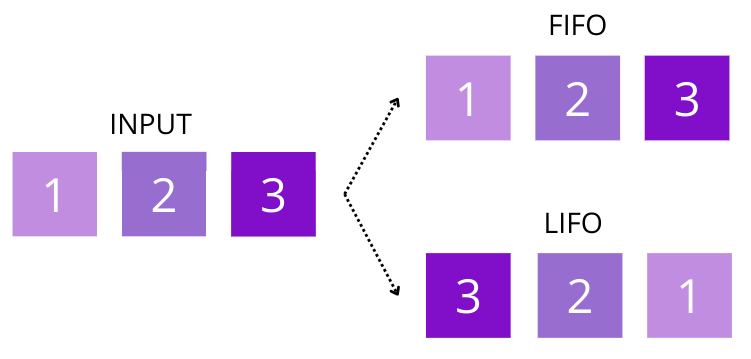
\includegraphics[width=0.5\linewidth]{Imagenes/Software/FIFO.jpg}
                        \caption{Cómo funciona FIFO y LIFO}
                        \label{fig:s1}
                    \end{figure}

                    En  nuestro programa, utilizamos colas FIFO para interconectar ambos núcleos, declarando un acceso directo a la entrada de la cola desde el \texttt{core\_0}, por ejemplo, en conjunto con otro acceso a la salida de dicha cola en el \texttt{core\_1}. No hay superposición entre los registros de ambos núcleos, por lo tanto puede funcionar de forma correcta.\par
	                Las colas FIFO las podemos utilizar desde nuestro programa aprovechando las funciones:\par
                    \texttt{void multicore\_fifo\_push\_blocking(uint32\_t data);}\par
                    Esta función es la que agrega un parámetro de formato (uint32\_t data) a la cola.\par
                    \texttt{uint32\_t multicore\_fifo\_pop\_blocking();}\par
                    Esta función es la que luego lo recogerá, para almacenarlo en una variable del mismo tipo.\par
                
        \section{Desarrollo del Servidor Web}
            \subsection{Introducción}
                La finalidad de nuestro proyecto incluye la confección de una aplicación web que se actualice en tiempo real en función de los datos obtenidos en el sistema de control.\par
                Aprovechando el manejo de FreeRTOS del \texttt{core\_0} del microcontrolador, designamos una tarea para realizar la transferencia de datos desde el sistema hacia el Servidor Web, desde donde la Aplicación Móvil levantará los datos necesarios para brindar la información que consideramos pertinente para el usuario.\par
            
            \subsection{Módulo ESP8266-01}
                Para generar el Servidor Web, utilizamos una ESP8266 01, un módulo wifi de la familia ESP.\par
                Este módulo permite 3 modos de funcionamiento:\par
                
                \begin{enumerate}
                \setlength{\itemindent}{1.5em}
                    \item \textbf{Modo AP (\textit{Access Point})}, donde el módulo crea su propia red WiFi, a la que otros dispositivos pueden conectarse directamente. (Es útil para entornos sin una red existente u offline).
                    \item \textbf{Modo STA (\textit{Station})}, donde el módulo se conecta a una red WiFi ya existente. Este modo le permite al módulo acceder a internet y ser accesible desde otros dispositivos en la misma red.
                    \item \textbf{Modo Dual}, donde el módulo puede funcionar en AP y STA simultáneamente, permitiendo que otros dispositivos se conecten a su red mientras él se conecta al router para internet.
                \end{enumerate}
                
                Para la confección del servidor web podríamos trabajar con el modo AP o STA, nosotros elegimos el modo STA, donde el sistema solicita los datos de una red WiFi.\par
                
                \lstinputlisting[language=C++, firstline=132, lastline=132]{main.cpp}\par
                
                Para luego obtener la configuración ip del router\par

                \lstinputlisting[language=C++, firstline=140, lastline=140]{main.cpp}\par
                
                La ESP8266 01 cuenta con un puerto de comunicación serial del tipo \textbf{UART} (\textit{Universal Asynchronous Receiver-Transmitter}), un protocolo caracterizado por su gran cantidad de ventajas frente a otros modos.\par
                Únicamente requiere dos pines, transmisor y receptor (TX y RX).\par
                No utiliza una arquitectura \textit{master/slave} (maestro/esclavo), como si es el caso de los protocolos I2C o SPI.\par
                No necesita un \textit{clock} durante la comunicación. Siendo este el canal que más complicaciones puede causar a grandes distancias debido a los retardos o a su sensibilidad ante las interferencias electromagnéticas, el protocolo UART nos resguarda de todas estas problemáticas al permitirnos la comunicación a través de grandes distancias o zonas con mucha interferencia electromagnética.\par
                Se trata de un protocolo que cuenta con estándares de bajo nivel, esto nos asegura que haya una gran cantidad de dispositivos, incluyendo a aquellos más antiguos, puedan comunicarse con el módulo.\par
                El protocolo UART es un protocolo de comunicación Full-Duplex, donde ambos dispositivos pueden enviar y recibir datos en ambos sentidos y en simultáneo. Esto se destaca del protocolo I2C (que cuenta con comunicación Half-Duplex, que permite comunicación bidireccional, pero no avala ambas en simultáneo), y del protocolo SPI (que también cuenta con Half-Duplex pero este requiere un reloj adicional).\par
                A continuación una tabla donde se especifican ventajas y desventajas de cada uno de los tipos de comunicación, considerando la cantidad de pines que requiere cada uno, la necesidad de un reloj externo o clock, la velocidad máxima que pueden utilizar, el grado de complejidad que presentan, el modo de transmisión, la cantidad de dispositivos que permiten:\par

                \begin{table}[H]
                    \centering
                    \begin{tabular}{|c|c|c|c|}
                        \hline
                         Característica & UART & I2C & SPI\\
                        \hline
                         Pines necesarios & 2 & 2 + GND & 4 + GND\\
                        \hline
                        Reloj externo & No & Sí & Sí\\
                        \hline
                        Velocidad máxima & \~1 Mbps & \~3,4 Mbps & \~10 Mbps\\
                        \hline
                        Complejidad & Baja & Media & Alta\\
                        \hline
                        Número de dispositivos & 2 & Hasta 127 (direcciones) & Maestro + varios esclavos\\
                        \hline
                        Modo de transmisión & Full-Duplex & Half-Duplex & Full-Duplex\\
                        \hline
                    \end{tabular}
                    \caption{Ventajas y Desventajas de Communicaciones}
                    \label{tab:s6}
                \end{table}
                
                Si  bien el protocolo de comunicación predefinido para la ESP8266 01 es el UART, este módulo nos permite emular otros protocolos de comunicación serial como I2C, SPI o el uso de puertos uart adicionales. Estas opciones no son recomendables por las limitaciones que presentan en velocidad y fiabilidad.\par
                Para más información sobre este componente en concreto revisar el Apéndice C, y más específicamente la Figura C.4.\par
                
            \subsection{Programa Principal}
                El módulo ESP8266-01 cuenta con un programa instalado, el main.cpp. Este será el primero que ejecutará el módulo al recibir alimentación y la orden de inicio.
            	Este programa es el encargado de recibir los datos recibidos desde la RP2040-Zero vía UART para enviarlos luego al mismo servidor web que inicia, donde solicitará los datos la app móvil.\par
            	Los datos enviados se encuentran codificados dentro de una cadena del tipo JSON, combinando valores con cadenas de texto para mejorar la comprensión de los datos. A penas son recibidos, son decodificados para extraer los valores y ubicarlos en su espacio correspondiente.\par
            	El módulo cuenta con 5 variables declaradas dentro, cada vez que recibe un dato vía UART actualiza el contenido de cada uno de ellos.\par
            	En simultáneo, está pendiente a pedidos del tipo GET:\par
                
                \lstinputlisting[language=C++, firstline=90, lastline=90]{main.cpp}
                
                Esta es la solicitud que envía la aplicación móvil al servidor web. Luego de recibir cada una de ellas, el servidor envía en respuesta otra cadena codificada con los datos, ya preparados para ser utilizados por la app móvil.
                Esta misma puede solicitar por separado los datos de cada uno de los sensores, acción que consideramos conveniente durante el desarrollo de este sistema.\par
                El módem WiFi le asigna a la ESP8266-01 una dirección IP, misma a la que se dirigirá la app móvil para efectuar la comunicación. Para que esta sea exitosa, ambos dispositivos deben estar utilizando la misma red WiFi, ya que esta designación es netamente local. Por este motivo, el uso de la aplicación será óptimo desde dentro del mismo domicilio o propiedad en la que fue instalada la batería.
                Para asegurar la actualización constante de los datos para la aplicación, manteniendo las lecturas del usuario renovadas en tiempo real, el microcontrolador cuenta con una tarea de FreeRTOS que envía datos regularmente. Es de muy baja prioridad, la que más baja tiene el sistema, pero aún así resulta óptimo para la recepción de datos desde el servidor.\par